\documentclass[12pt]{article}

%PACKAGES
\usepackage{graphicx}
\usepackage{epstopdf}
\usepackage[english]{babel}
\usepackage[toc,page]{appendix}
\usepackage{listings}
\usepackage{caption}
\usepackage{epsfig}

\usepackage{hyperref}
\usepackage[left=3cm,top=3cm,right=3cm,nohead,nofoot]{geometry}
\usepackage{braket}
\usepackage{datenumber}
\usepackage{placeins}


%COMMANDS

\begin{document}

\begin{center}
\begin{figure}
\centering%
\epsfig{file=logo-andes.jpg,scale=0.75}%
\end{figure}
\vspace{3 cm}
\FloatBarrier
\Huge
Laniakea in a Cosmological Context\\
\vspace{3 mm}
or\\
\vspace{3 mm}
Detection of galaxy superclusters in simulated cosmological structures\\  
\vspace{1 cm}
\vspace{3mm}
\Large Sergio Daniel Hern\'{a}ndez Charpak\\

\large
200922618\\
\vspace{1 cm}
\vspace{2mm}
\Large
Advisor: Jaime E. Forero-Romero\\

\normalsize
\vspace{2mm}
\vspace{1 cm}
\today \\
\vspace{1 cm}
\small 
Universidad de los Andes\\
Facultad de Ciencias, Departamento de F\'{i}sica\\
Bogot\'{a}, Colombia\\
\end{center}


\normalsize
\newpage
\section{Acknowledgements}

I would like to thank my advisor, Jaime E. Forero-Romero, for his guidance
 during this process, of course my family, Nathalie, Jose Tiberio, Yv\'{a}n David,
  Gabriel Luis, Nico, Dani and all the others for
   their great patience and always good advices. I
    also acknowledge the University of Los Andes
     for its mayor financial support during my
      studies. Finally I couldn't have finish this
       without the support of Andr\'{e}s,
        Nicol\'{a}s, Jorge and all the special
         friends I am lucky to have.


\newpage
\section{Abstract}
Recently Tully et al. (2014)
 \cite{tully_laniakea_2014} used local cosmic flow
 information to define our local supercluster,
  Laniakea. 
In this work we present a study on large
 cosmological N-body
simulations aimed at establishing the significance
 of Laniakea in a
cosmological context.
We explore different algorithms to define
 superclusters from the dark
matter velocity field in the simulation. 
We summarize the properties of the supercluster
 population by their
abundance at a given total mass and its shape
 distributions.
We find that superclusters similar in size and
 structure to Laniakea are
relatively uncommon on a broader cosmological
 context.
We finalize by discussing the possible sources of
 systematics (both in
our methods and in observations) leading to this
 discrepancy.
%TODO make sure it is what it is
\newpage
\tableofcontents
\newpage

\section{Introduction}

In the Universe scene at large scales the galaxy group themselves in structures
similar to a filament web which go through large voids regions and cross in regions
called superclusters. Even though these structures can be easily detected at simple
view, there are different possibilities to delimited them from physical criteria \cite{gott_iii_map_2005}.    
\\

A proposal to define a supercluster is to use the flow of galaxy in this region of
space. Within a supercluster, galaxy tend to flow to the most dense region as a
consequence of the gravitational attraction process. In this way, spacial regions where
the galaxy flow is convergent represent galaxy superclusters.\\
\\
Recently a team build a galaxy velocities flow map of the local group in a scale of
hundreds of light years \cite{tully_cosmicflows-2_2013}. In this map converging points
were found and this team identified Laniakea, the galaxy supercluster which includes
our galaxy, the milky way \cite{tully_laniakea_2014}.
\\   

We propose to develop a method to detect a
 statistical significant number of galaxy
supercluster in cosmological simulations. 
With this we aim to quantify if Laniakea can be
 considered as an atypical structure in
the Universe. 
\\

\section{Background}
\subsection{Cosmic flows and peculiar velocities}
%Describe in detail the Laniakea work and the Methods used
The peculiar velocity refers to the velocity relative to a rest frame. In the case of the
Cosmicflows-2 map, the rest frame is the earth. 
The Laniakea supercluster of galaxy was mainly identified following an analysis of the
peculiar velocities flows. A Wiener filtering method was apply to obtained a better
Signal/Noise proportion and separate the peculiar velocities from the cosmic expansion.\\
%TODO Explain how the fieltering worked




\subsection{Boundaries of Laniakea - The V-Web Algorithm}
\label{sec:v_web}
The contour of the region were reconstructed with
 the V-web Algorithm. This algorithm is deeply
  connected to the velocities as its core is the
   shear velocity tensor.\\

%TODO Explain how the V-Web algorithm worked. 


\subsection{Fractional Anisotropy and Overdensity}
\label{sec:FA_trace}
\section{Methods}

As we support the open-source community, we used the N-Body simulation open
software Gadget-2 \cite{springel_gadget_2_2005} to generate the simulations
and source code in C and Python to treat the data obtained from the
simulations. The development of the code will be in Github \url{https://github.com/sercharpak/Monografia/}.

\subsection{Simulations}
We used the N-Body simulation software Gadget-2
 \cite{springel_gadget_2_2005}
widely used in the scientific community to
 generate different boxes of dark matter particles
  (DM). The initial conditions were
generated with Springel's N-Genic software. The
 simulations ran on the HPC cluster at UNIANDES.
  The main properties (boxsize, number of
   particles, number of CPUs used and time of the
    simulation) are described in table
     \ref{tab:sims}. \\

\begin{table}[ht]
    \centering
    \begin{tabular}{|c|c|c|c|}
        Boxsize [Mpc/h] & DM particles & \# CPU & Time [hours] \\
        500 & $512^{3}$ & 48 & \~ 10 \\
        250 & $512^{3}$ & 48 & \~ 6  \\
        500 & $1024^{3}$ & 48 & \~ 70  \\
    \end{tabular}
    \caption{Different Gadget-2 Simulations}
    \label{tab:sims}
\end{table}
\FloatBarrier

By DM particle we mean a particle which only
 interacts through gravity
interaction. In the simulation each particle
 represents a galaxy. The DM particles are
placed in a 3D grid layout first and then are
 perturbed following Poisson distribution
before the simulation start, during the initial
 conditions generation.\\

Once the simulation starts, the particles interact
 only with gravity as time goes by following the
  cosmological constants. Here these were not
   modified, the default values were used.\\

We then use different algorithms to identify the
 superclusters within the simulation.\\

\subsection{Approaches}
%Opening the section

\subsubsection{Naive: the magnitude of the velocity}
\label{sec:naive_speed}
\begin{par}
In a first approach we analyse the distribution of
 the magnitude of the velocity in the different
  simulations. We work with all the particles and
   points given by the simulation. As our final
    results are not based in this naive approach
     we leave it as an appendix here. It is
      explained in further detail in Appendix
       \ref{App:App_Speed}.
\end{par}

\subsubsection{More complete: V-Web, CIC, the FA and $\delta$}

\begin{par}
In our second approach, we used directly the V-Web
 algorithm to form the Fractional Anisotropy (FA)
  and the Overdensity $\delta$) to have detailed
   results comparable to Laniakea's.\\
Finally we apply a Cloud In Cell (CIC) method and
 a Gaussian smooth to have a more manipulable grid
  to work with.\\
\end{par}


\begin{par}
We described the V-Web algorithm in section
 \ref{sec:v_web}. Let us remind the velocity shear
  tensor as 
%TODO write the velocity shear tensor
\end{par}

\begin{par}
The CIC method is used to transform the box to a
 grid in which the (i,j,k) have {$\lambda_1$,
  $\lambda_2$, $\lambda_3$} values related to the
   number of particles in a cell.
%TODO explain in detail de CIC and gaussian smooth.
Each cell has a number of particles in it and
 hence a total mass equivalent to the sum of the
  mass of its particles.
\end{par}

\begin{par}
And in section \ref{sec:FA_trace} we saw how the
 FA and $\delta$ are formed and are relevant in
  this context. 
%TODO maybe expand this a little bit
We are then looking for regions with $\delta$
 positive and FA lesser than 1.0.
%TODO the lesser than 1.0 could be rephrased.
\end{par}

%Closing the section
\begin{par}
Our approach is hence very close with the approach
 used to define Laniakea
  \cite{tully_laniakea_2014} which is important to
   validate our later comparison of Laniakea with
    our detected structures.
\end{par}

\subsection{Algorithms}

Our main algorithm is a region growing algorithm
 as described by Gonzalez
  \cite{gonzalez_digital_2008} mainly used in
   image segmentation. We now proceed to describe
    it generally.

\subsubsection{Region Growing Algorithm: General Description}

%TODO General description of the algorithm as described by Gonzalez







\subsubsection{Region Growing Algorithm with the FA and Overdensity}
Our implementation is based in the FA and the Overdensity $\delta$.
%TODO Describe my implementation

\subsubsection{Region Growing Algorithm and FoF with the FA and Overdensity}
Finally we improved this last method making used of the Friends-of-Friends (FoF) algorithm.
%TODO Describe the FoF and the final pipeline implementation





\section{Results}


\subsection{Region Growing Algorithm with the FA and Overdensity}

\subsection{Region Growing Algorithm and FoF with the FA and Overdensity}

\subsection{Comparisons with Laniakea}

\section{Conclusions}

%TODO The Future Work section needs to be re-written
\section{Future Work}
\begin{itemize}
	\item Understand more in detail how the work done by Hoffman et al\cite{hoffman_kinematic_2012} in the V-web algorithm, was used to determine Laniakea.
    \item Write our own Gadget-2 snapshop reader in C or Python which implements the region growing algorithm.
    \item Optimize our Algorithm. The current results are not sufficient.
    \item Run a bigger simulation (boxsize: $5 \times 10^{6} Mpc/h$ and $1024^3$ DM particles.
    \item Run the algorithm on this simulation.
    \item Compare the properties of the results with the Laniakea supercluster.
    \item Discuss the sources of systematics in both methods and observations.
\end{itemize}



\bibliographystyle{unsrt}
%\renewcommand\refname{Referencias}
\bibliography{references}

\appendix
\section{Approach by the Speed} \label{App:App_Speed}
\subsection{Region Growing Algorithm with the Speed}

We present here a naive way to approach to the problem. 
\begin{enumerate}
	\item We calculate the magnitude of the velocity (the speed) of each particle. 
	\item We look for regions where the center has the highest speed and from it the speed decreases while the particle is further away from the center. 
    \item We define the limits of this region the regions where the speed begins to increase with the distance from the center.
\end{enumerate}

\begin{par}
We use a region growing algorithm, a simple image segmentation algorithm
used to identify different regions in a image \cite{gonzalez_digital_2008}.
\end{par}

\begin{par}
$f(x,y,z)$ denotes the input data. $S(x,y,z)$ denotes a seed array, with
value 1 where the particle can be define as a seed and 0 where not. It is the
same size of $f(x,y,z)$. $Q$ denotes a predicate which is to be apply to the
input data and determines if the region which
 starts at the seeds grows or
not. Here $Q$ denotes: "if the speed of the close
 particle is lower than the
marked one but greater than a threshold, mark that
 particle and continue."
\end{par}

\begin{enumerate}
	\item We choose seeds to begin the growth. In
	 this case we choose the particles with high
	  velocities. Here \[ |v|>  th_{high}\]
	\item We open a window of particles to look
	 for 2 close particles from the seed $s$ which
	  do not for part of $S(x,y,z)$. Here:
    \[ window = 20000\]
    \item Once we found the 2 close particles $c$ we apply the predicate $Q$. Here:
    \[ Q := |v_s| > |v_c| > |th_{low}|\]
    
    \item If the particle $c$ satisfies $Q$, it is
     marked, $S(c) = 1$
    \item Apply the algorithm to $c$, and so on
     (Recursion).
\end{enumerate}

Here we defined empirically different thresholds
 in order to observer the results. \\
First we used:  \\
$th_{low} = v_{min} + \frac{\sigma_{v}}{2} $ and
 $th_{high} = v_{max}  - \sigma_{v}$ .\\
Secondly we used: \\
$th_{low} = \vec{v} + 2  \sigma_{v} $ and $th_{high} = \vec{v}  +  8 \sigma_{v}$.\\

The first version of the algorithm was written in
 python using the module
pyGadgetReader
 \cite{thompson_pygadgetreader_2014ascl_soft11001T}
  to read the
data and transform it to NumPy arrays in Python.
 In Appendix \ref{App:App_speed_code} we attach
  the source code used.

\subsection{Results of the Speed Approach}
This approach was tested on the simulation of
 boxsize 500 Mpc/h
and $512^{3}$ dark matter particles (DM) described
 in table \ref{tab:sims}. \\

We first visualize the speed histogram in figure
 \ref{fg:hist_vel}.\\

%Speed histogram
\begin{figure}[ht]
\begin{center}
\includegraphics[width=0.9\textwidth]{graphs/hist_vel.png} % Include the image placeholder.png
\caption{Speed Histogram of the simulation}
\label{fg:hist_vel}
\end{center}
\end{figure}
\FloatBarrier

The histogram resembles a Poisson distribution. This is a consequence of the perturbations generated in the initial conditions generation. 

\begin{table}[ht]
    \centering
    \begin{tabular}{|c|c|}
        $v_{max}$ & 2023.87 \\
        $v_{min}$ & 0.34\\
        $\sigma_{v}$ & 117.75 
    \end{tabular}
    \caption{Properties of the speed distribution}
    \label{tab:vel}
\end{table}
\FloatBarrier

Our hypothesis is based on the most direct implication of gravity. The lower speed
particles will mainly be in the border regions and the higher speed particles
will be in the center regions. \\

For this we must choose a threshold for low velocities and a threshold for high velocities. 
We obtain: $th_{low} = v_{min} + \frac{\sigma_{v}}{2} = 59.2$ and $th_{high} = v_{max}  - \sigma_{v} = 1906.12 $

%Plot 3Ds
%First 3D plot, particles with speed lower than thresh_low
We first have a look at the particle distribution of particles with speed higher than the
threshold for low velocities.\\
%59.216707265
\begin{figure}[ht]
\begin{center}
\includegraphics[width=0.8\textwidth]{graphs/pos_3d_vel_menor_s_smaller.png} % Include the image placeholder.png
\caption{DM particles with $|v| < 59.2 $}
\label{fg:3d_thresh_low}
\end{center}
\end{figure}
\FloatBarrier

There seem to be some structures, but it is not clear enough. This is due to the high number of DM particles used in the simulation ($512^3$). 

%Second 3D plot, particles with speed higher than thresh_high

We produce cuts in the z-direction to visualize in 2-D the speed distribution. \\

%Plot 2D

%5 plots of the 2D. 
\begin{figure}[ht]
\centering
\begin{minipage}{.45\textwidth}
  \centering
  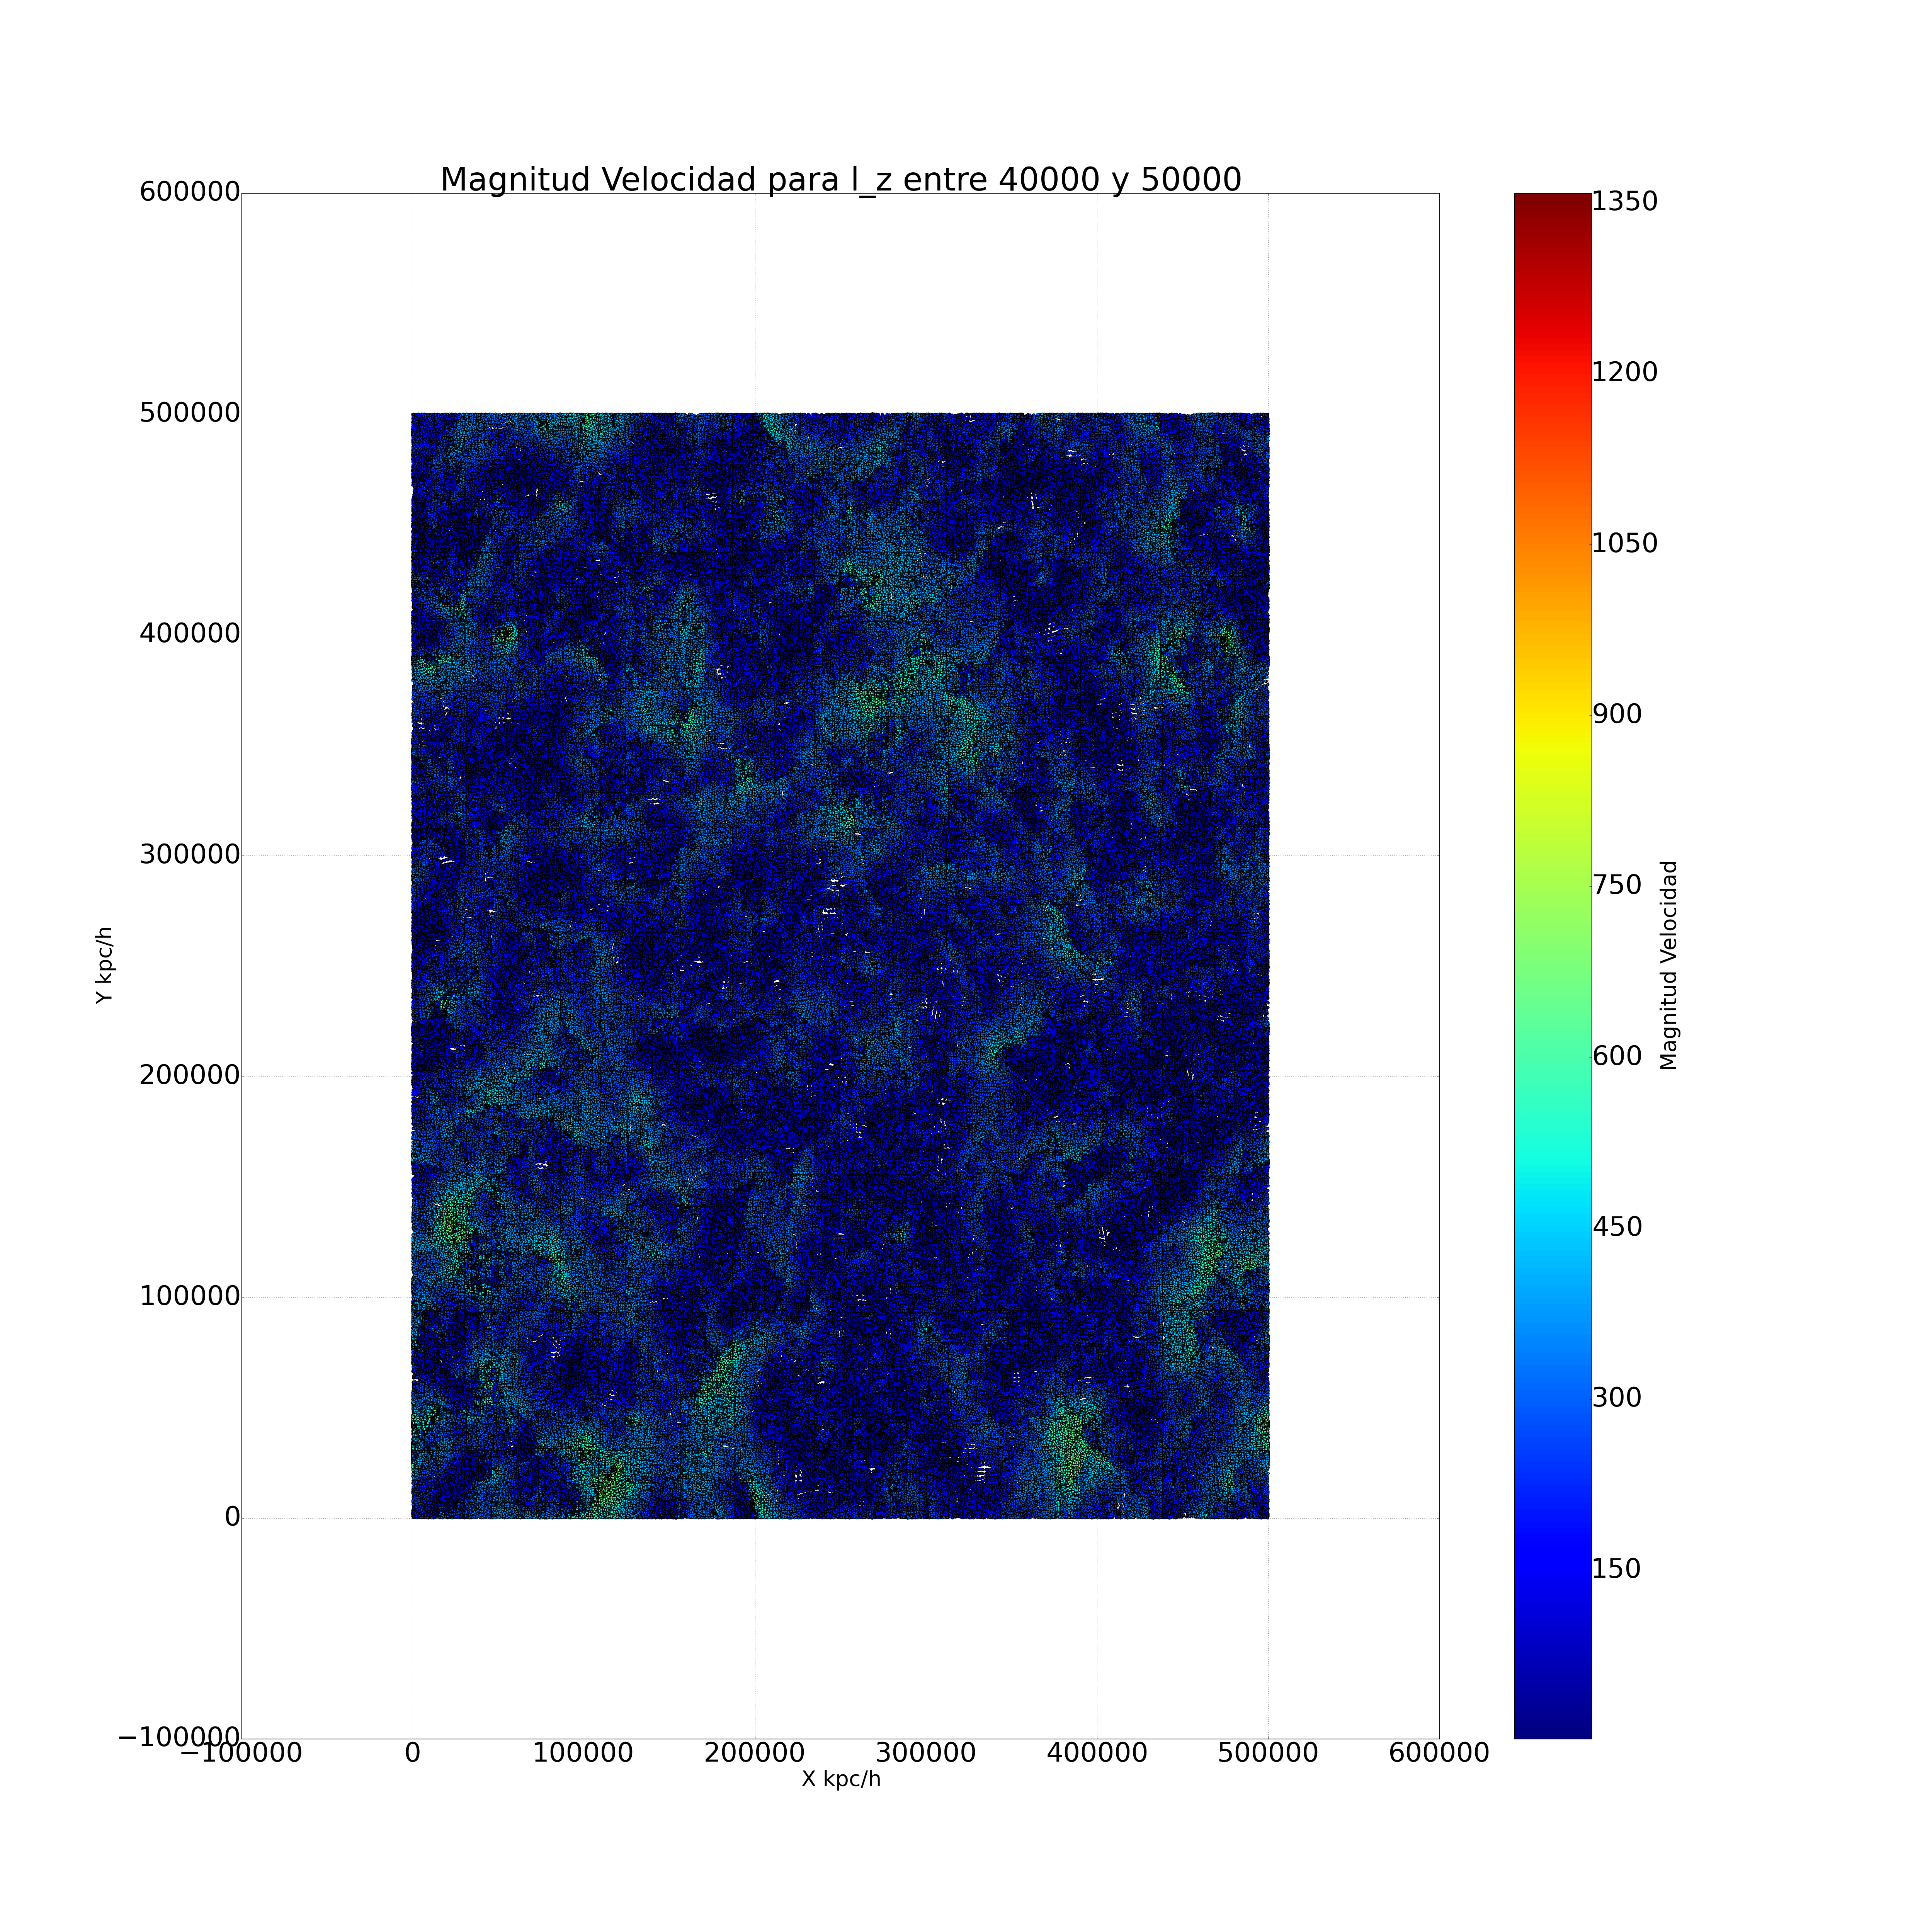
\includegraphics[width=0.9\textwidth]{graphs/scatter_magnitud_vel50000.png}
\end{minipage}%
\begin{minipage}{.45\textwidth}
  \centering
  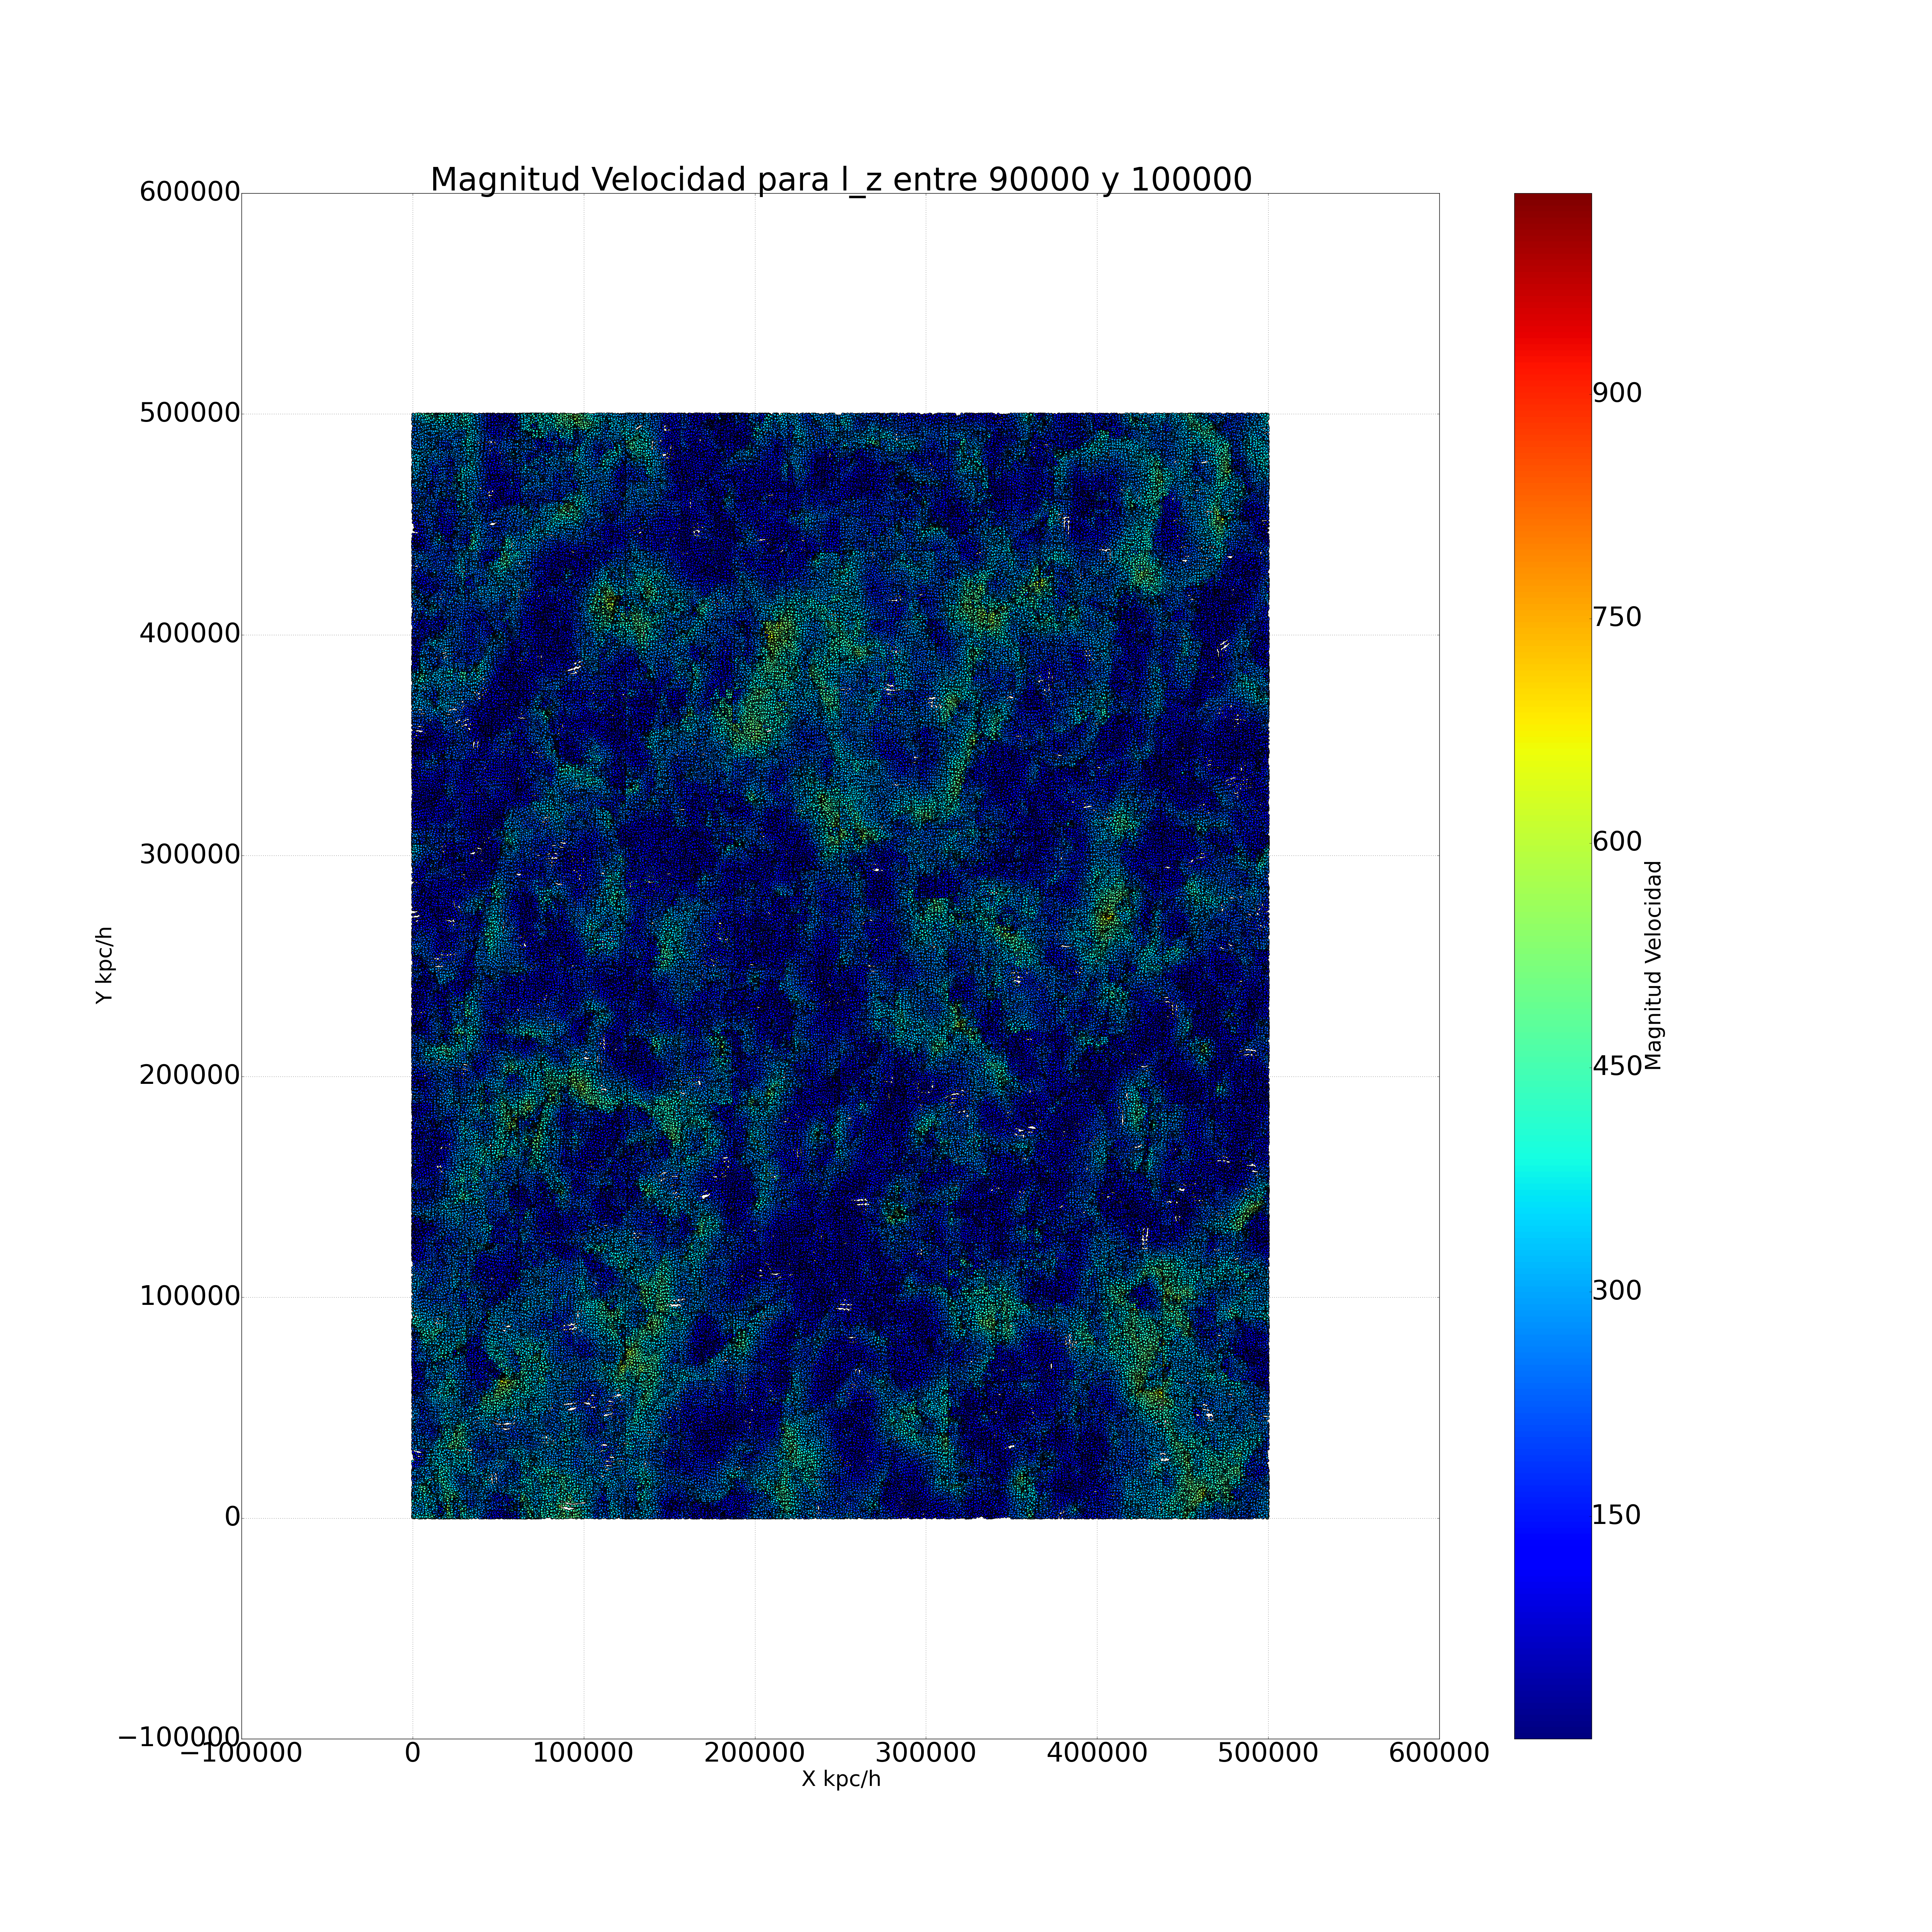
\includegraphics[width=0.9\textwidth]{graphs/scatter_magnitud_vel100000.png}
\end{minipage}
\begin{minipage}{.45\textwidth}
  \centering
  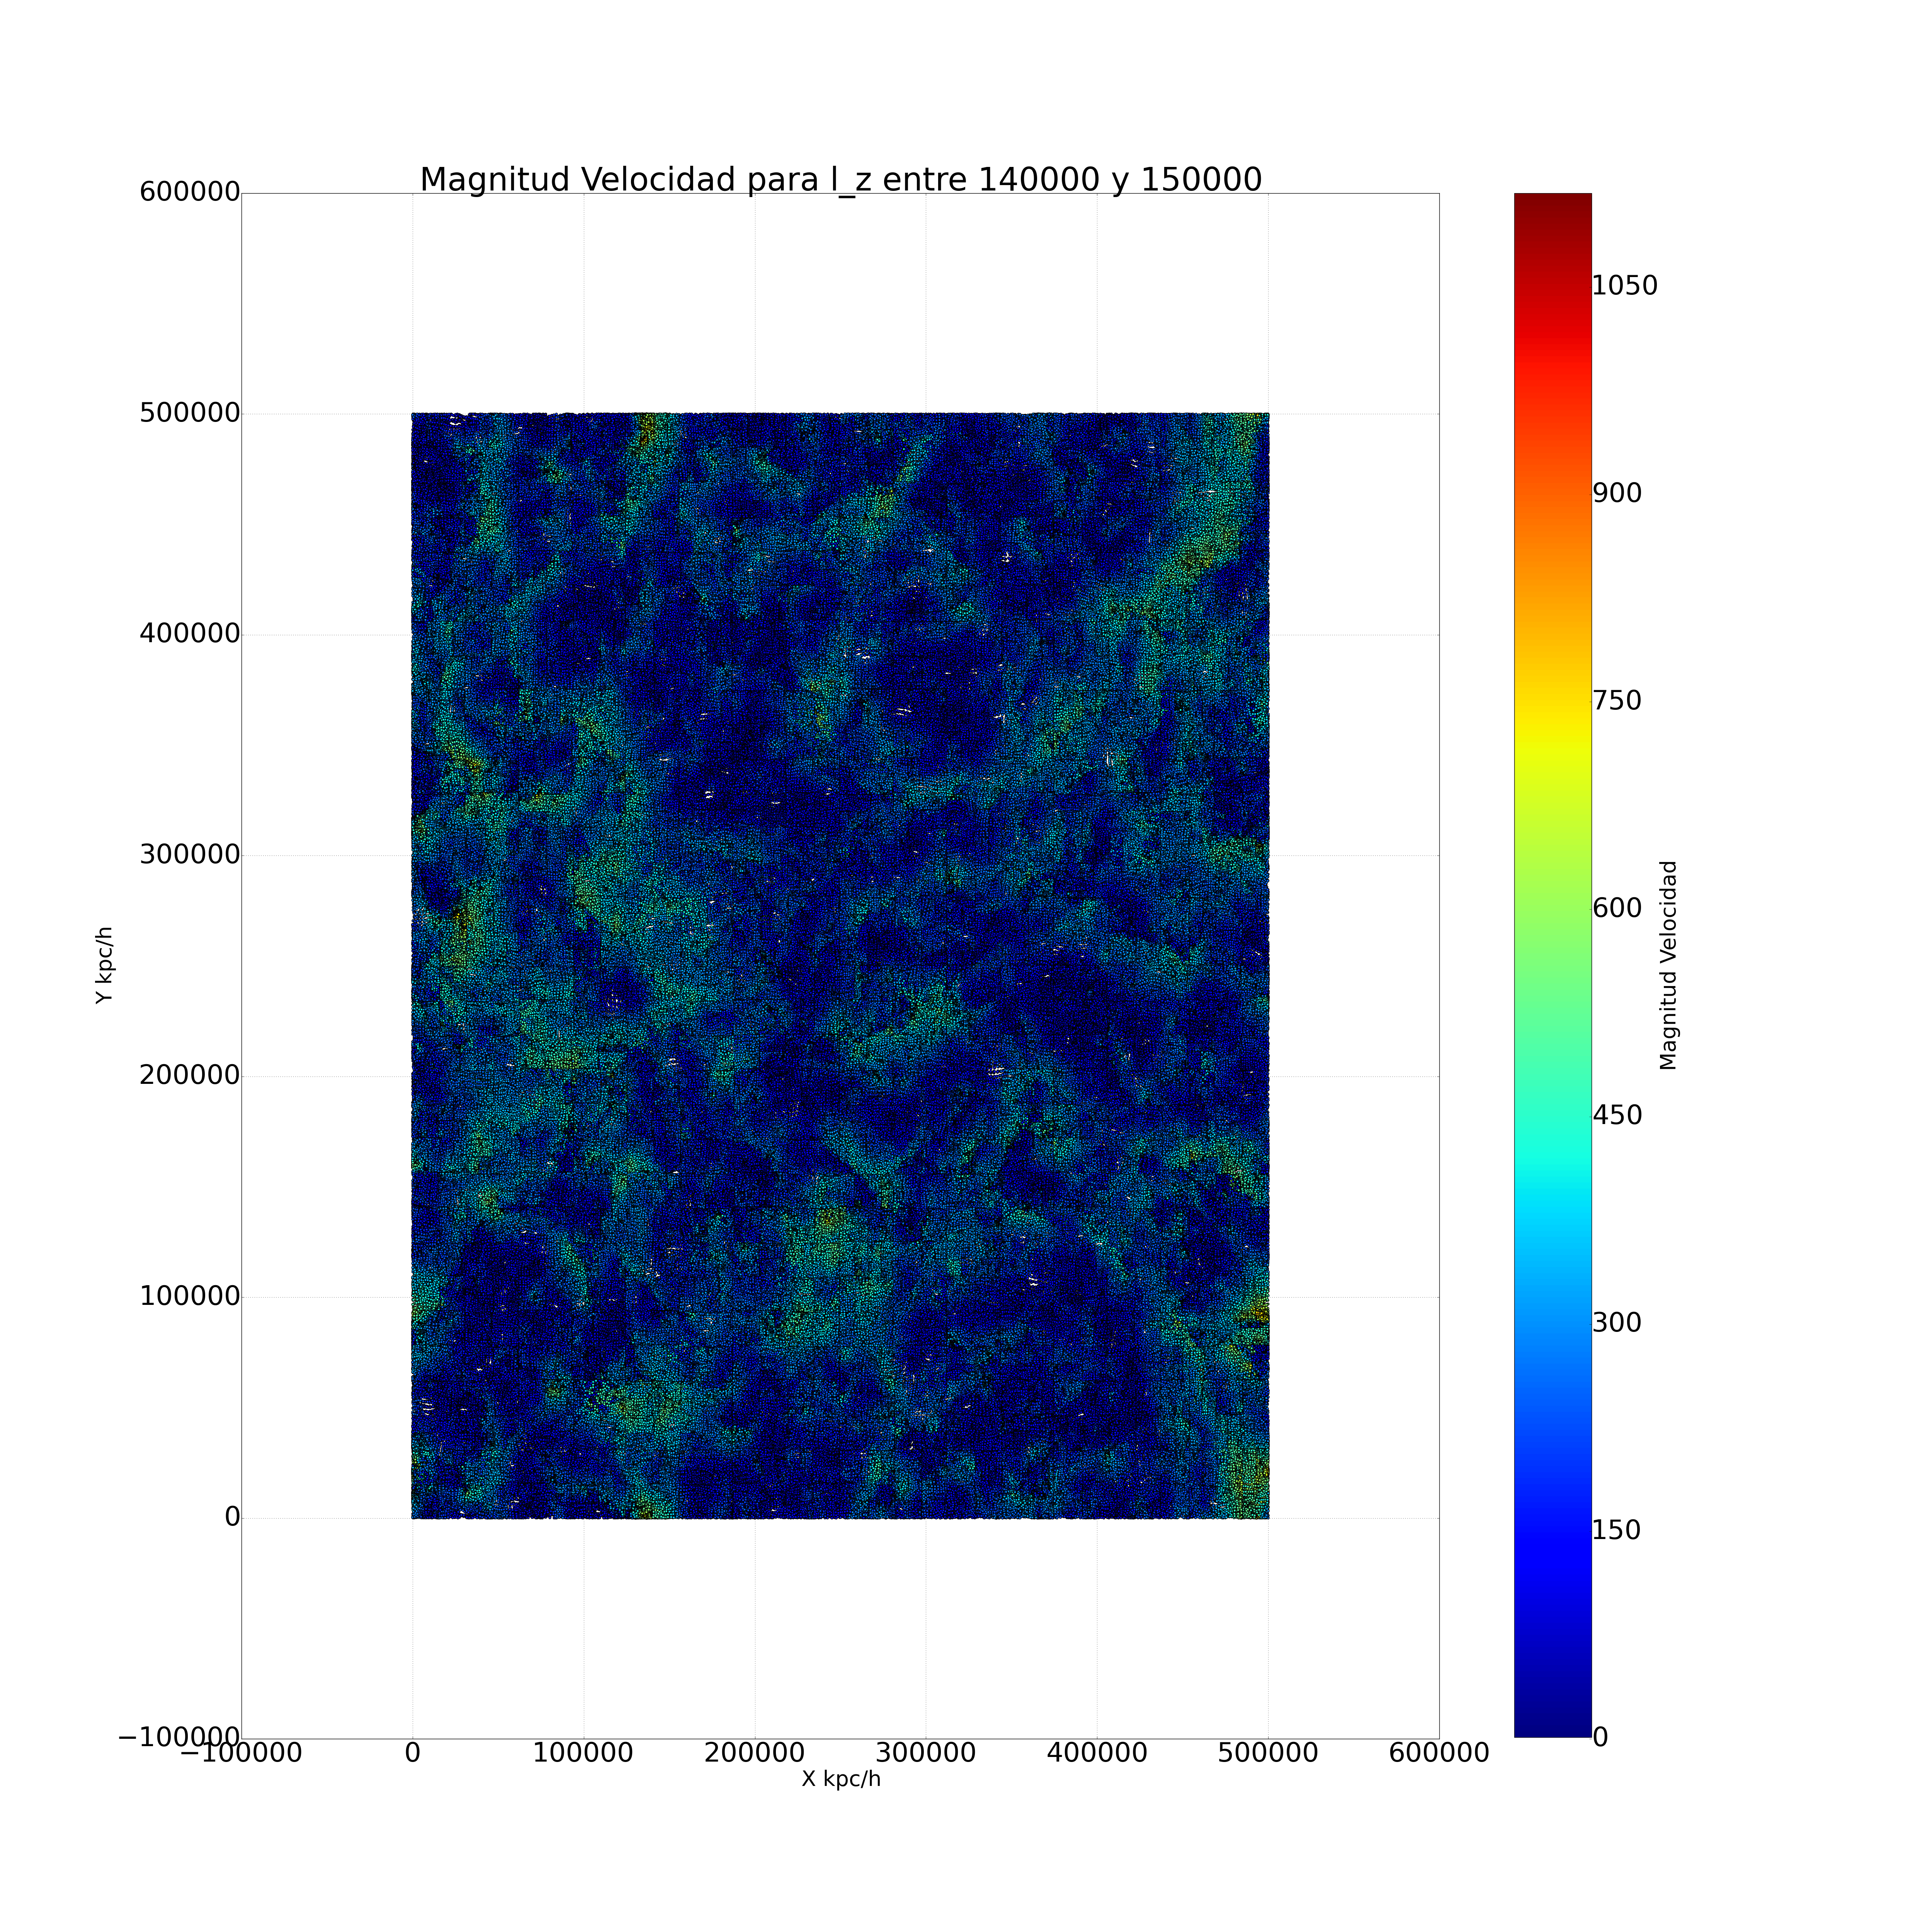
\includegraphics[width=0.9\textwidth]{graphs/scatter_magnitud_vel150000.png}
\end{minipage}
\begin{minipage}{.45\textwidth}
  \centering
  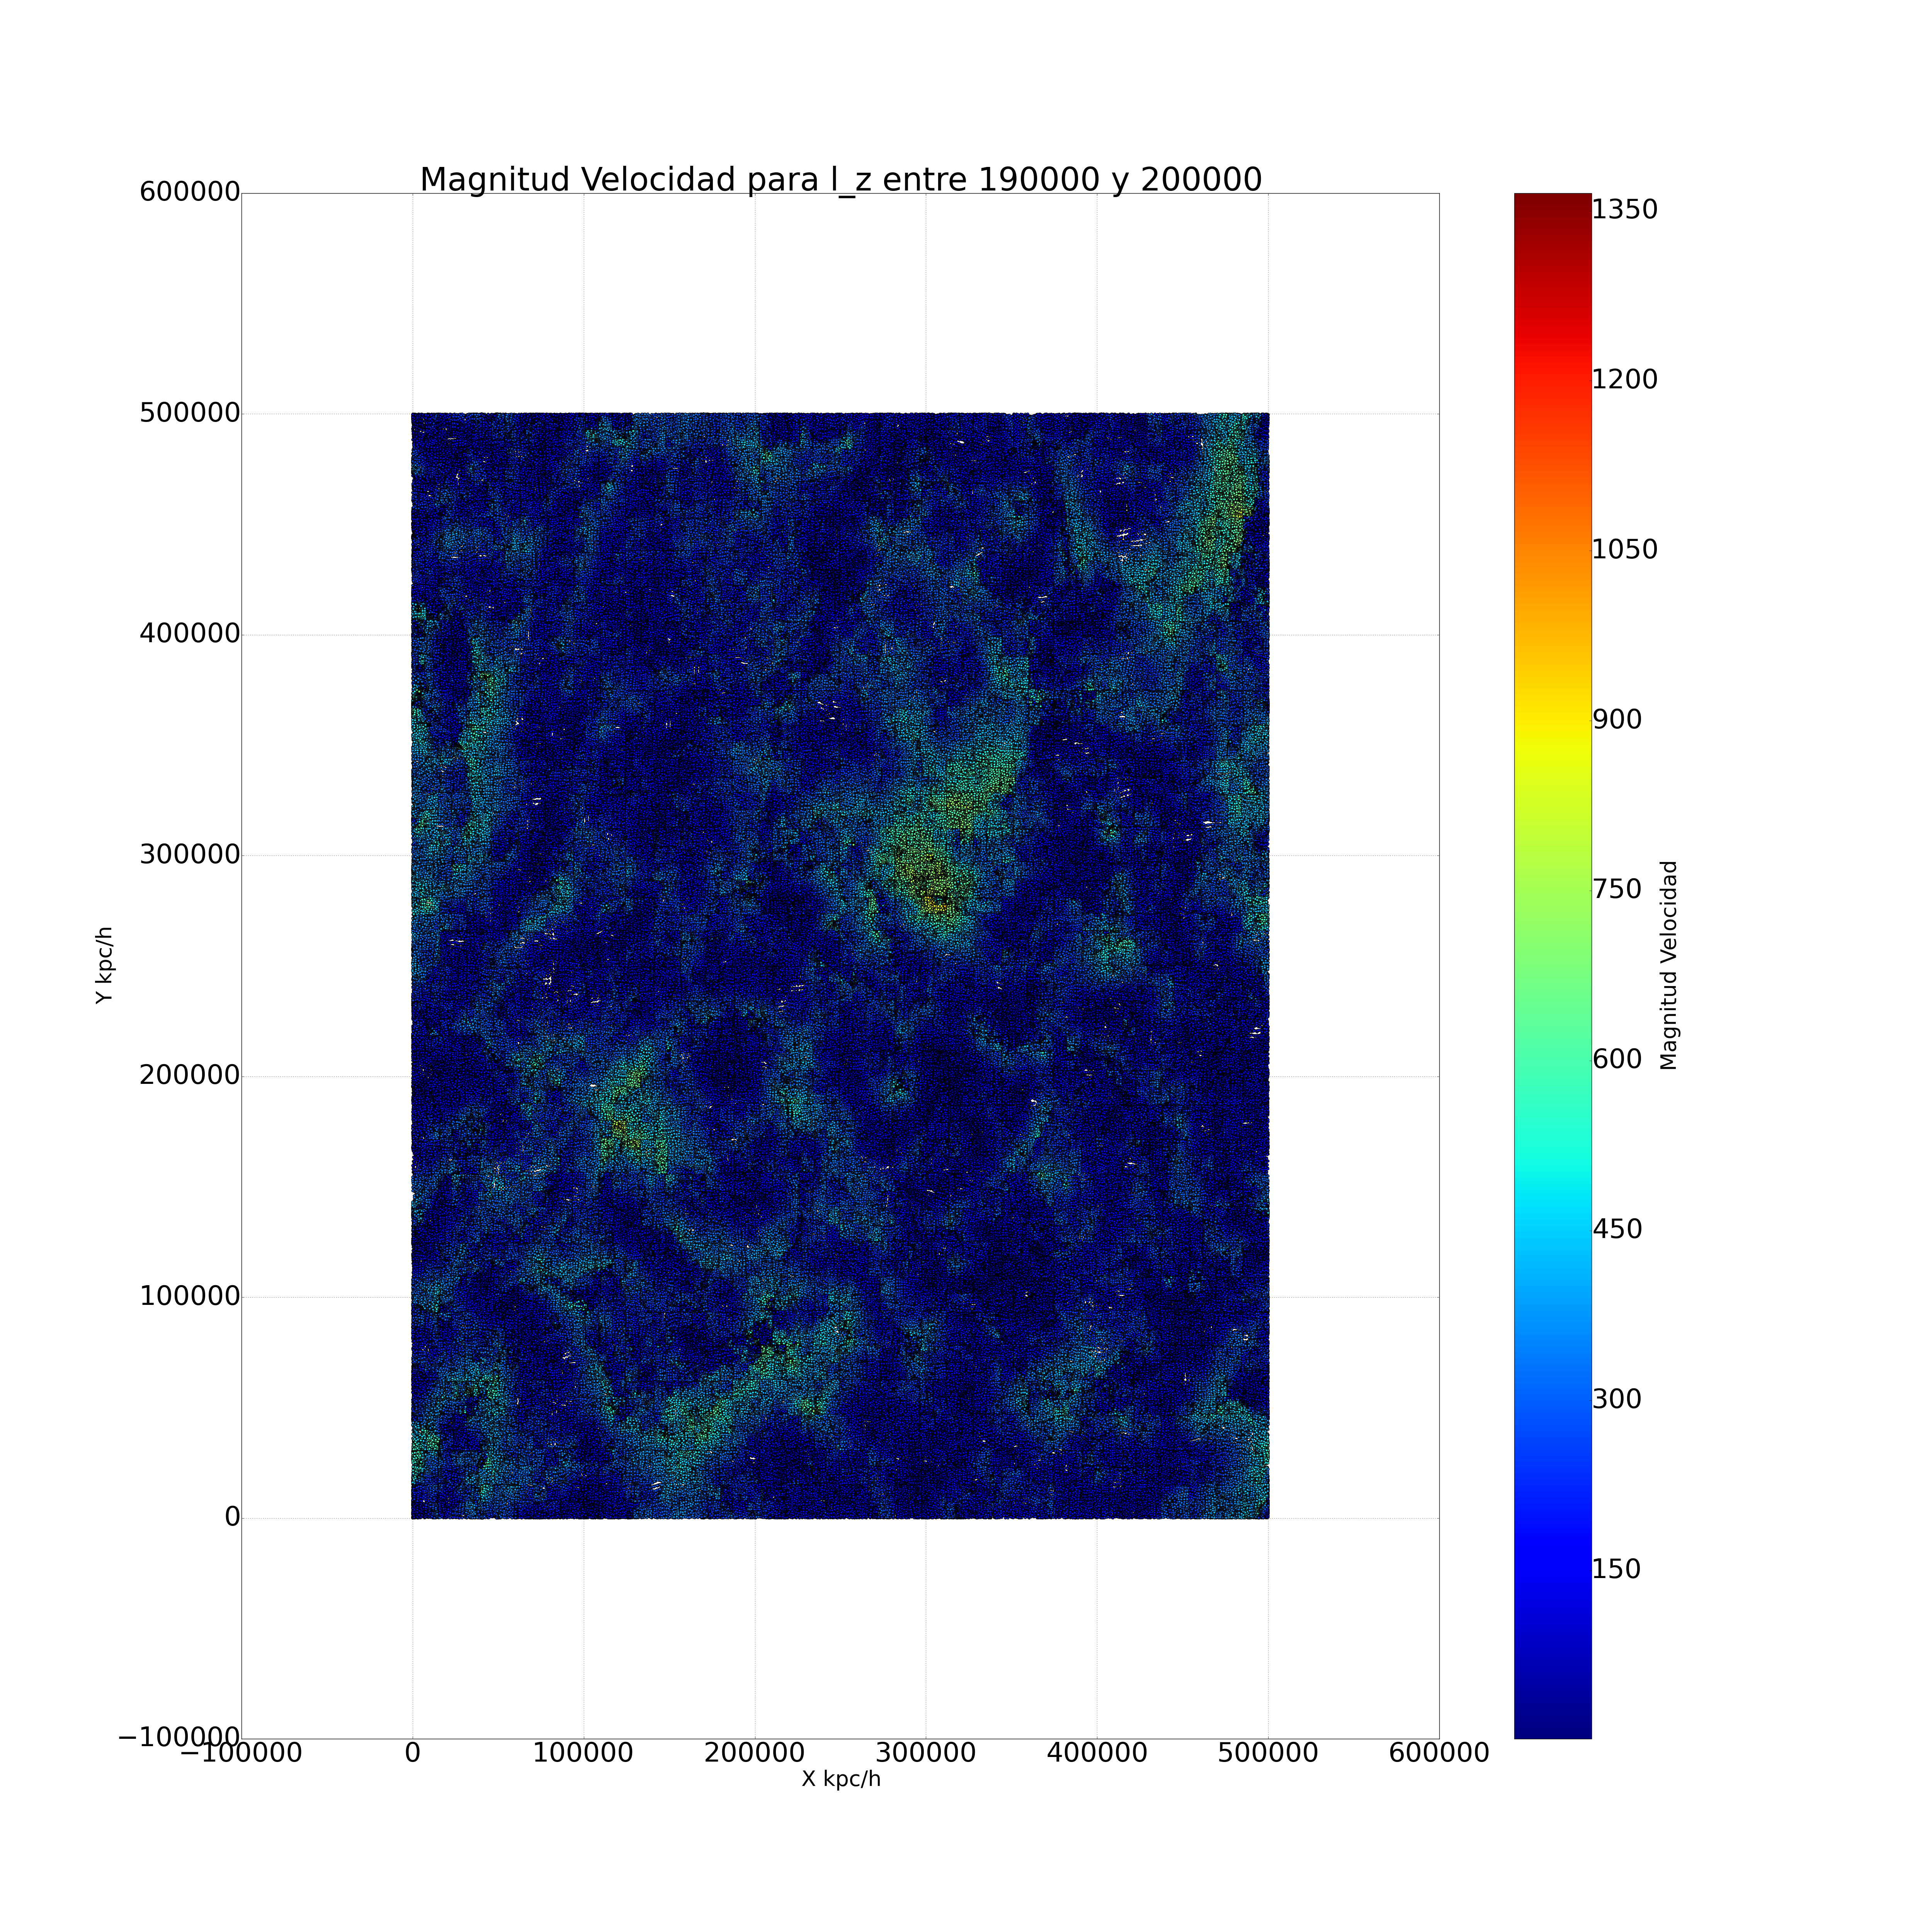
\includegraphics[width=0.9\textwidth]{graphs/scatter_magnitud_vel200000.png}
\end{minipage}
\caption{2D slices of the speed distribution}\label{fig:2D_slices}
\end{figure}
\FloatBarrier


We can observe in figure \ref{fig:2D_slices} intuitive signs of structures related to the speed distribution. 
We can observe filament structures\\

It is more clear if we observe from one side the particles with speed greater than a $th_{high}$ and the particles with speed lesser than a $th_{low}$.\\

\begin{figure}[ht]
\centering
\begin{minipage}{.45\textwidth}
  \centering
  \includegraphics[width=0.9\textwidth]{graphs/scatter_magnitud_vel_488_lz_100000.png}
\end{minipage}%
\begin{minipage}{.45\textwidth}
  \centering
  \includegraphics[width=0.9\textwidth]{graphs/scatter_magnitud_vel_488_lz_200000.png}
\end{minipage}
\begin{minipage}{.45\textwidth}
  \centering
  \includegraphics[width=0.9\textwidth]{graphs/scatter_magnitud_vel_59_lz_100000.png}
\end{minipage}
\begin{minipage}{.45\textwidth}
  \centering
  \includegraphics[width=0.9\textwidth]{graphs/scatter_magnitud_vel_59_lz_200000.png}
\end{minipage}
\caption{2D slices of the speed distribution. The upper slices with $|\vec{v}| > th_{high} = 488$ and the two lower slices with $|\vec{v}| < th_{low} = 59$ for the same cuts, $z = \{100, 200 \} Mpc/h$ and }\label{fig:2D_slices_thresh}
\end{figure}
\FloatBarrier

As we can see in figure \ref{fig:2D_slices_thresh} the cuts with low and high thresholds are complementary. It is evident that structures are present. 

Finally we apply our region growing algorithm and we obtain the following results.\\

%Plot of the region identified.
\begin{figure}[ht]
\begin{center}
\includegraphics[width=0.8\textwidth]{graphs/regions_small.png} % Include the image placeholder.png
\caption{Region identified by the algorithm}
\label{fg:regions_speed_th_1}
\end{center}
\end{figure}
\FloatBarrier

And, changing the thresholds to: 
$th_{low} = \bar{v} + 2  \sigma_{v} = 488.48$ and $th_{high} = \bar{v}  +  8 \sigma_{v} =1195.0 $\\
We obtain:
%Plot of the region identified.
\begin{figure}[ht]
\begin{center}
\includegraphics[width=0.8\textwidth]{graphs/regions_big.png} % Include the image placeholder.png
\caption{Region identified by the algorithm with the second thresholds}
\label{fg:regions_speed_th_2}
\end{center}
\end{figure}
\FloatBarrier

We have different observations:\\
\begin{enumerate}
	\item The details of the regions in figures \ref{fg:regions_speed_th_1} and \ref{fg:regions_speed_th_2} seem accurate with what we would expect. It is more dense in the center and less dense in the borders.
	\item The regions obtained have a dimension of only a few Mpc/h (Laniakea's dimension is two orders of magnitude higher). This could mean that Laniakea is atypical. 
    \item There is first only one region identified. This indicates than all the high velocity particles are congregated in only one region (the detected region). If we set lower $th_{high}$ we can see we get more regions. 
    \item This is certainly a good naive approach to the problem. Nevertheless for more accurate results it needs to be drastically changed.
\end{enumerate}

The script in Appendix \ref{App:App_speed_code} was executed in a student's
laptop and later on the HPC cluster. For a significant number of particles, the laptop limited memory (8GB) crashes. Running in the HPC solves this issue. results.


\subsection{Code example for Region Growing Algorithm - Approach by the Speed} \label{App:App_speed_code}
\tiny
\lstinputlisting[language=Python, caption=Region Growing Algorithm Code]{code/region_detection_document.py}
\end{document} 
